\chapter{Anexos}

\section{Generación de proyecto Petalinux} \label{petalinux}

El paquete de software de PetaLinux proporciona al usuario las herramientas para configurar, construir y desplegar todos los componentes de software necesarios en las plataformas de Xilinx, que son:
\begin{itemize}
  \item \acrshort{FSBL}
  \item U-Boot
  \item ARM Trusted Firmware (\acrshort{ATF})
  \item Linux
  \item Librerías y programas de usuario
  \item Hipervisor Xen
\end{itemize}


\subsection{Plataforma Hardware}
El primer paso para generar un proyecto de Petalinux es disponer de lo que en la nomenclatura Xilinx se denomina \textit{hardware platform specification}. Esta plataforma es el resultado de sintetizar el implementar el diseño definido en Vivado. Una vez que se ha generado el bitstream, se ha de exportar la plataforma, lo que genera un fichero \textit{.hdf} que contiene toda la información (configuración de \acrshort{PS} y bitstream para \acrshort{PL}) que necesitan las herramientas de Xilinx para poder desarrollar software.

\subsection{Creación de proyecto}
Es necesario cargar las variables de entorno necesarias a fin de poder utilizar las herramientas del paquete de software PetaLinux en el host. Para ello es necesario introducir el siguiente comando (el texto entre signos < > debe ser sustituido por lo que corresponda según la instalación):\\

\begin{lstlisting}[style=CStyle]
alex@xubuntu16:~/workspace/ultrazed_hyp_1$ source <ruta_hasta_instalacion_petalinux>/settings.sh
\end{lstlisting}

Una vez hecho esto, el proyecto PetaLinux se crea con el siguiente comando en el que se le indica la plataforma (zynqMP para los MPSoC) y el nombre del proyecto, ultrazed\_hyp\_1.

\begin{lstlisting}[style=CStyle]
alex@xubuntu16:~/workspace/ultrazed_hyp_1$ petalinux-create --type project --template zynqMP --name ultrazed_hyp_1
\end{lstlisting}


\subsection{Importar plataforma hardware}

Una vez está creado el proyecto, a fin de importar la plataforma hardware previamente generada con Vivado, se ejecuta lo siguiente en la shell:

\begin{lstlisting}[style=CStyle]
alex@xubuntu16:~/workspace/ultrazed_hyp_1$ petalinux-config --get-hw-description=<ruta_hasta_fichero_hdf_generado_por_vivado>
\end{lstlisting}

Si en el directorio especificado existe un fichero \textit{.hdf}, entonces PetaLinux importa toda la configuración que contiene y muestra una ventana como la de la figura \ref{fig:petalinux_config_1}, en la que permite al usuario modificar los parámetros para la generación de los binarios:\\

\begin{figure*}[!h]
	\centering
	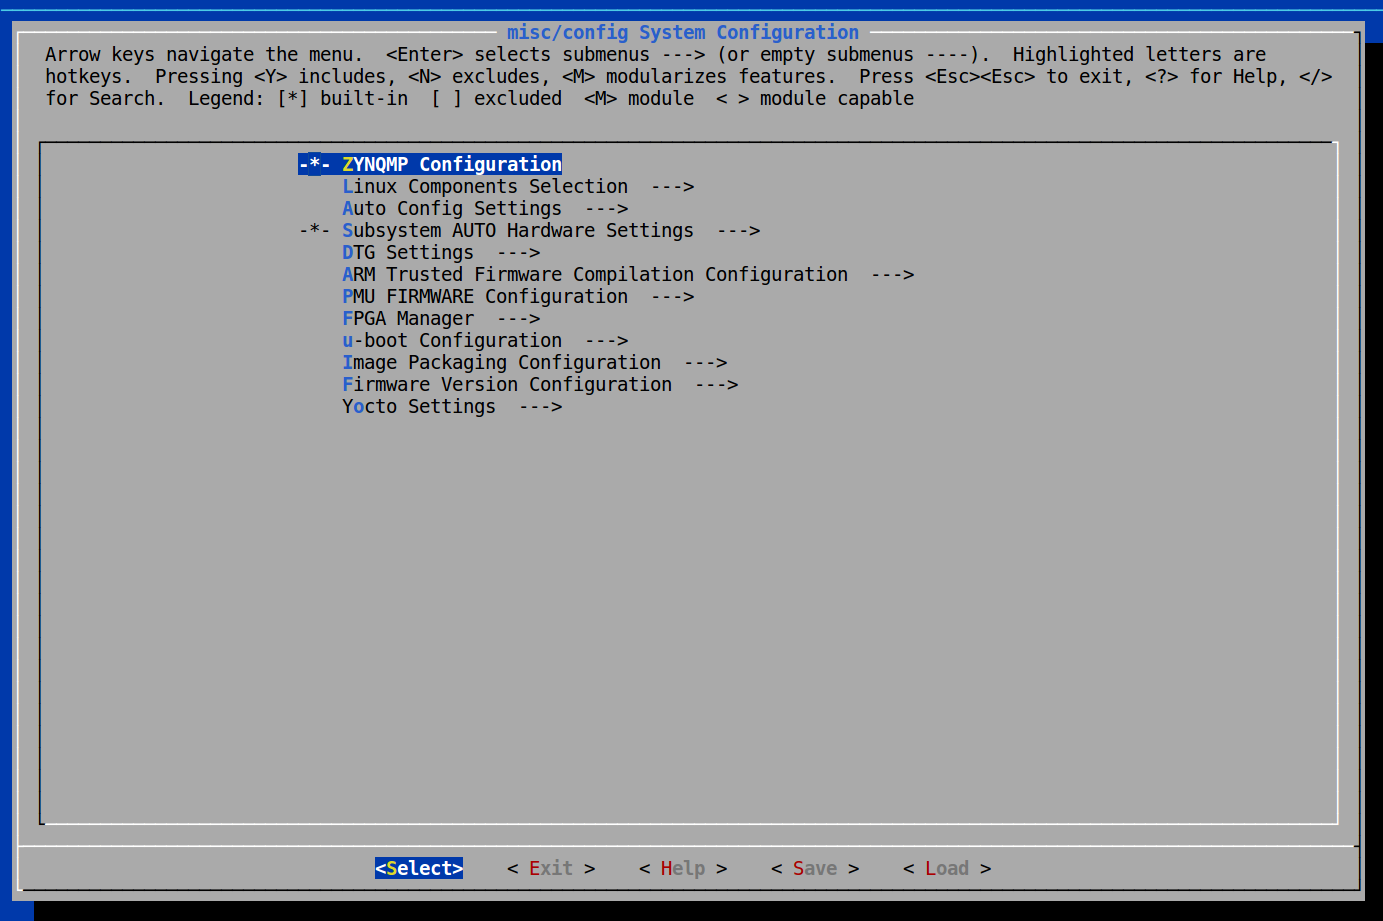
\includegraphics[width=0.95\textwidth]{recursos/petalinux_config_1.png}
	\caption{Configuración de proyecto PetaLinux}
	\label{fig:petalinux_config_1}
\end{figure*}

\subsection{Construcción del proyecto}

Después de configurar el proyecto a partir de la plataforma hardware, el siguiente paso es generar los binarios necesarios para el sistema. Petalinux crea una estructura de directorios dentro del proyecto que tiene el siguiente aspecto:\\

\begin{lstlisting}[style=CStyle]
project-spec
 meta-plnx-generated
 hw-description
 configs
 meta-user
pre-built
 linux
 implementation
 images
hardware
 xilinx-zcu104-2019.1
components
 plnx_workspace
 device-tree
config.project
README
README.hw
\end{lstlisting}

Dentro de esta estructura, se generan automáticamente una serie de ficheros dependiendo de la definición de la plataforma hardware importada desde Vivado. Por ejemplo, existe un fichero \textit{pl.dtsi} en el que se incluyen los nodos del \textit{device-tree} de los dispositivos metidos en la zona de \textit{PL}.\\
Petalinux dedica la carpeta \textit{meta-user} a las modificaciones que el usuario quiera realizar a los valores por defecto del proyecto. Es en este lugar donde se puede por ejemplo cambiar configuraciones de kernel de Linux, aplicar parches a paquetes de software, o hacer cambios en el \textit{device-tree}.

Para generar los binarios del proyecto, se introduce el siguiente comando:

\begin{lstlisting}[style=CStyle]
alex@xubuntu16:~/workspace/ultrazed_hyp_1$ petalinux-build
\end{lstlisting}

El proceso de generación tarda un tiempo considerable ya que descarga y compila para la plataforma una gran cantidad de software. Como resultado del proceso, en la carpeta \textit{images/linux/} almacena todos los binarios compilados:

\begin{lstlisting}[style=CStyle]
alex@xubuntu16:~/workspace/ultrazed_hyp_1/images/linux$ ls -l
total 1783116
-rw-r--r-- 1 alex alex     51744 Aug 15 20:14 bl31.bin
-rw-r--r-- 1 alex alex    154488 Aug 15 20:14 bl31.elf
-rw-rw-r-- 1 alex alex   6659824 Aug 15 21:54 BOOT.BIN
-rw-r--r-- 1 alex alex  14901760 Aug 15 22:18 Image
-rw-r--r-- 1 alex alex   7120904 Aug 15 22:19 image.ub
-rw-r--r-- 1 alex alex    140504 Aug 15 20:16 pmufw.elf
-rw-r--r-- 1 alex alex  82912288 Aug 15 10:59 rootfs.bin
-rw-r--r-- 1 alex alex 228598784 Aug 15 22:23 rootfs.cpio
-rw-r--r-- 1 alex alex  68484524 Aug 15 22:23 rootfs.cpio.bz2
-rw-r--r-- 1 alex alex  75789385 Aug 15 22:24 rootfs.cpio.gz
-rw-r--r-- 1 alex alex  75789449 Aug 15 22:24 rootfs.cpio.gz.u-boot
-rw-r--r-- 1 alex alex 321724416 Aug 15 22:23 rootfs.ext3
-rw-r--r-- 1 alex alex  69201590 Aug 15 22:23 rootfs.ext3.bz2
-rw-r--r-- 1 alex alex 321724416 Aug 15 22:23 rootfs.ext4
-rw-r--r-- 1 alex alex  76002955 Aug 15 22:24 rootfs.ext4.gz
-rw-r--r-- 1 alex alex      2250 Aug 15 10:59 rootfs.its
-rw-r--r-- 1 alex alex 100139008 Aug 15 22:24 rootfs.jffs2
-rw-r--r-- 1 alex alex     14954 Aug 15 22:23 rootfs.manifest
-rw-r--r-- 1 alex alex  68550268 Aug 15 22:23 rootfs.tar.bz2
-rw-r--r-- 1 alex alex  76015225 Aug 15 22:24 rootfs.tar.gz
-rw-r--r-- 1 alex alex    301693 Aug 15 22:23 rootfs.testdata.json
-rw-r--r-- 1 alex alex   5568788 Aug 15 20:03 system.bit
-rw-r--r-- 1 alex alex     35100 Aug 15 22:18 system.dtb
-rw-r--r-- 1 alex alex   3348212 Aug 15 22:19 System.map.linux
-rw-r--r-- 1 alex alex    795072 Aug 15 22:19 u-boot.bin
-rw-r--r-- 1 alex alex    861400 Aug 15 22:19 u-boot.elf
-rw-r--r-- 1 alex alex 220059496 Aug 15 22:19 vmlinux
-rw-r--r-- 1 alex alex    121984 Aug 15 20:16 zynqmp_fsbl.elf
\end{lstlisting}


\subsection{Generar sistema de arranque}

El proceso de arranque de un chip de la familia MPSoC se detalla en \cite{axi_trm}. Los componentes necesarios y un ejemplo de arranque típico se muestran en la figura \ref{fig:mpsoc_boot}.

\begin{figure*}[!h]
	\centering
	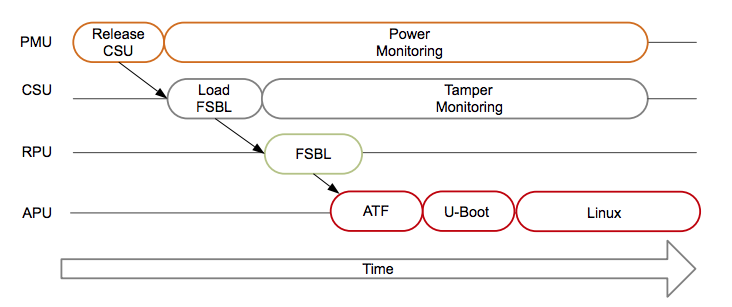
\includegraphics[width=0.95\textwidth]{recursos/mpsoc_boot.png}
	\caption{Configuración de proyecto PetaLinux}
	\label{fig:mpsoc_boot}
\end{figure*}


En el caso de la UltraZed\texttrademark, para la mayoría de los tests se arranca desde la tarjeta microSD. En esta tarjeta hay dos particiones: una con los ficheros necesarios para el arranque, y otra con el sistema de ficheros.\\

Los binarios generados en el paso anterior se agrupan en un fichero \textit{BOOT.BIN} con \acrshort{FSBL}, \acrshort{ATF}, bitstream y U-Boot, y un \textit{image.ub} con la imagen del kernel y el \textit{device-tree}. Estos dos ficheros se guardan en la primera partición de la tarjeta microSD y son los que arrancan el sistema hasta el kernel.

Para generar el fichero \textit{BOOT.BIN} es necesario ejecutar el siguiente comando de PetaLinux:

\begin{lstlisting}[style=CStyle]
alex@xubuntu16:~/workspace/ultrazed_hyp_1$ petalinux-package --boot --fsbl --fpga --uboot
\end{lstlisting}
